\documentclass[t]{beamer}

\mode<presentation>
{
    \usetheme{rwthsimple}
    \setbeamercovered{transparent = 0}
}

\setbeamertemplate{section in toc shaded}[default][30]
\setbeamertemplate{subsection in toc shaded}[default][30]

% \pgfplotsset{compat=1.9}

\usepackage{caption}
\usepackage{algorithm}
\usepackage{algorithmic}
\usepackage{xspace}
\usepackage{enumitem}
\usepackage{subcaption}
\usepackage{pgfplots}
\usepackage{tikz}

% http://tex.stackexchange.com/questions/18325/disable-the-numbering-of-algorithms
\renewcommand{\thealgorithm}{}

\pgfplotsset{every tick label/.append style={font=\scriptsize},every axis/.append style={legend style={font=\scriptsize}}}

% http://tex.stackexchange.com/questions/57117/algorithms-package-ignores-caption-package
% \captionsetup[algorithm]{font=small}

% http://tex.stackexchange.com/questions/4728/how-do-i-number-equations-only-if-they-are-referred-to-in-the-text
%\usepackage{mathtools}
%\mathtoolsset{showonlyrefs=true}
\usepackage{autonum}

\makeatletter
\DeclareRobustCommand\onedot{\futurelet\@let@token\@onedot}
\def\@onedot{\ifx\@let@token.\else.\null\fi\xspace}
\def\eg{{e.g}\onedot} \def\Eg{{E.g}\onedot}
\def\ie{{i.e}\onedot} \def\Ie{{I.e}\onedot}
\def\cf{{c.f}\onedot} \def\Cf{{C.f}\onedot}
\def\etc{{etc}\onedot} \def\vs{{vs}\onedot}
\def\wrt{w.r.t\onedot} \def\dof{d.o.f\onedot}
\def\etal{{et al}\onedot}

% proximal map operator
\DeclareRobustCommand{\prox}[1]{%
    \ifmmode
        \text{prox}_{#1}
    \else
        $\text{prox}_{#1}$
    \fi
}
\def\dom{\text{dom}}
\def\per{\text{per}}

\title{iPiano: Inertial Proximal Algorithm for Non-Convex Optimization}

\author{David Stutz}
\RWTHtoc{Table of Contents}

\newcommand\blfootnote[1]{%
    \begingroup
    \renewcommand\thefootnote{}\footnote{#1}%
    \addtocounter{footnote}{-1}%
    \endgroup
}

\begin{document}
	\RWTHtitle
	
	\section{Problem}
	\begin{frame}{Problem}
		\textbf{Problem.} Minimize composite function
		\begin{align}
			\min_{x \in \mathbb{R}^d} h(x) = \min_{n \in \mathbb{R}^d} (f(x) + g(x))\only<2>{\begin{tikzpicture}[overlay]\draw[-,thick,RWTHblue] (0.1,-0.45) -- (-5.25,-0.45) -- (-5.25,0.65) -- (0.25,0.65) -- (0.25,-0.45);\end{tikzpicture}}\label{eq:problem}
		\end{align}
		where
		\begin{enumerate}[label=--]
			\pause
			\item $f : \mathbb{R}^d \rightarrow \mathbb{R} \in C^1$ with $L$-Lipschitz continuous gradient;
			\pause
			\item $g : \dom(g) \subset \mathbb{R}^d \rightarrow \mathbb{R}_\infty$ is proper closed convex and lower semicontinuous;
			\pause
			\item and $h$ coercive and bounded below by
			\begin{align}
				-\infty < h_{\min} := \inf_{x \in \mathbb{R}^d} h(x).
			\end{align}
		\end{enumerate}
		
		\pause
		Ochs \etal \cite{OchsChenBroxPock:2013} combine forward-backward splitting with an inertial force/momentum term to solve Equation \eqref{eq:problem} iteratively.
	\end{frame}
	
	\section{Related Work}
	\begin{frame}{Related Work}
		Gradient descent for $h \in C^1$:
		\begin{align}
			x^{(n + 1)} = x^{(n)} - \alpha_n \nabla h(x^{(n)})\only<2>{\begin{tikzpicture}[overlay]\draw[-,thick,RWTHblue] (0.25,-0.45) -- (-4.75,-0.45) -- (-4.75,0.65) -- (0.25,0.65) -- (0.25,-0.45);\end{tikzpicture}}.
		\end{align}
		Gradient descent with inertial force/momentum term:
		\begin{align}
			x^{(n + 1)} = x^{(n)} - \alpha_n \nabla h(x^{(n)}) + \beta_n(x^{(n)} - x^{(n - 1)})\only<3>{\begin{tikzpicture}[overlay]\draw[-,thick,RWTHblue] (0.25,-0.45) -- (-8.1,-0.45) -- (-8.1,0.65) -- (0.25,0.65) -- (0.25,-0.45);\end{tikzpicture}}.
		\end{align}
		Proximal point for $h$ being proper closed convex:
		\begin{align}
			x^{(n + 1)} = \prox{\alpha_n h} (x^{(n)})\only<4>{\begin{tikzpicture}[overlay]\draw[-,thick,RWTHblue] (0.25,-0.45) -- (-3.95,-0.45) -- (-3.95,0.65) -- (0.25,0.65) -- (0.25,-0.45);\end{tikzpicture}}.
		\end{align}
		Forward-backward splitting for $h = f + g$ with $f \in C^1$ and $f$, $g$ being proper closed convex:
		\begin{align}
			x^{(n + 1)} = \prox{\alpha_n g}(x^{(n)} - \alpha_n \nabla f(x^{(n)}))\only<5>{\begin{tikzpicture}[overlay]\draw[-,thick,RWTHblue] (0.25,-0.45) -- (-6.35,-0.45) -- (-6.35,0.65) -- (0.25,0.65) -- (0.25,-0.45);\end{tikzpicture}}.
		\end{align}
	\end{frame}
	
	\section{Algorithm}
	\begin{frame}{Algorithm -- Iterates and Backtracking}
		Ochs \etal \cite{OchsChenBroxPock:2013} combine forward-backward splitting with an inertial force/momentum term\only<1>{.}\only<2>{:}
		\pause
		\begin{align}
			x^{(n + 1)} = \prox{\alpha_n g}(x^{(n)} - \alpha_n \nabla f(x^{(n)}) + \beta_n(x^{(n)} - x^{(n - 1)}))\only<2>{\begin{tikzpicture}[overlay]\draw[-,thick,RWTHblue] (0.25,-0.45) -- (-9.75,-0.45) -- (-9.75,0.65) -- (0.25,0.65) -- (0.25,-0.45);\end{tikzpicture}}\label{eq:iteration}
		\end{align}
		with step size parameters $(\alpha_n)_{n \in \mathbb{N}}$ and momentum parameters $(\beta_n)_{n \in \mathbb{N}}$.
		\vskip 1em
		
		\pause
		Backtracking to estimate the local Lipschitz constant $L_n$ such that
		\begin{align}
			\begin{aligned}
				f(x^{(n + 1)}) \leq f(x^{(n)}) + &\nabla f(x^{(n)})^T (x^{(n + 1)} - x^{(n)})\only<4>{\begin{tikzpicture}[overlay]\draw[-,thick,RWTHblue] (0.25,-1.35) -- (-8,-1.35) -- (-8,0.65) -- (0.25,0.65) -- (0.25,-1.35);\end{tikzpicture}}\\
				+ &\frac{L_n}{2} \|x^{(n + 1)} - x^{(n)}\|_2^2
			\end{aligned}\label{eq:lipschitz-condition}
		\end{align}
	\end{frame}
	
	\begin{frame}{Algorithm -- iPiano}
		\begin{algorithm}[H]
			{
			\caption{iPiano.}
			\label{alg:ipiano}
			\begin{algorithmic}[1]
				\STATE{choose $c_1, c_2 > 0$ close to zero,  $L_{-1} > 0$, $\eta > 1$, $x^{(0)}$}
				\STATE{$x^{(-1)} := x^{(0)}$}
				\FOR{$n = 1, \ldots$}
					\only<1-2>{\STATE{ }}\only<3>{\STATE{$L_n := \frac{1}{\eta} L_{n - 1}$}\label{line:ipiano-backtracking}}
					\only<1-2>{\STATE{ }}\only<3>{\REPEAT}
						\only<1-2>{\STATE{ }}\only<3>{\STATE{$L_n := \eta L_n$}\label{line:ipiano-L}}
						\only<1>{\STATE{ }}\only<2-3>{\REPEAT}
							\STATE{choose $\alpha_n \geq c_1$, $\beta_n \geq 0$}\label{line:ipiano}
							%\STATE{$\delta_n := \frac{1}{\alpha_n} - \frac{L_n}{2} - \frac{\beta_n}{2\alpha_n}$}
							%\STATE{$\gamma_n := \frac{1}{\alpha_n} - \frac{L_n}{2} - \frac{\beta_n}{\alpha_n}$}
						\only<1>{\STATE{ }}\only<2-3>{\UNTIL{$\delta_n := \frac{1}{\alpha_n} - \frac{L_n}{2} - \frac{\beta_n}{2\alpha_n} \geq \gamma_n := \frac{1}{\alpha_n} - \frac{L_n}{2} - \frac{\beta_n}{\alpha_n} \geq c_2$}}
						\STATE{$x^{(n + 1)} = {\prox {\alpha_n g}} \left(x^{(n)} - \alpha_n \nabla f(x^{(n)}) + \beta_n (x^{(n)} - x^{(n - 1)})\right)$}
					\only<1-2>{\STATE{ }}\only<3>{\UNTIL{\eqref{eq:lipschitz-condition} is satisifed for $x^{(n + 1)}$}}
				\ENDFOR
			\end{algorithmic}
			}
		\end{algorithm}
	\end{frame}
	
	\begin{frame}{Algorithm -- Monotonically Decreasing $\delta_n$}
		\begin{lemma}
			For each $n \in \mathbb{N}$, given $L_n > 0$, there exist $\alpha_n < 2(1 - \beta_n)/L_n$ and $0 \leq \beta_n < 1$ as in iPiano such that $c_2 \leq \gamma_n \leq \delta_n$ and $(\delta_n)_{n \in \mathbb{N}}$ is monotonically decreasing.
		\end{lemma}
		
		\pause
		\begin{proof}[Proof Sketch.]
			With $b_n := (\delta_{n - 1} + \frac{L_n}{2})/(c_2 + \frac{L_n}{2})$:
			\begin{align}
				\gamma_n &\geq c_2 \text{ }\Leftrightarrow\text{ } \alpha_n \leq \frac{1 - \beta_n}{c_2 + \frac{L_n}{2}} < \frac{2(1 - \beta_n)}{L_n}\\
				\delta_{n - 1} &\geq \delta_n \text{ }\Leftrightarrow\text{ } \frac{1 - \beta_n}{c_2 + \frac{L_n}{2}} \geq \alpha_n \geq \frac{1 - \frac{\beta_n}{2}}{\delta_{n - 1} + \frac{L_n}{2}}\text{ }\Rightarrow\text{ } \beta_n \leq \frac{b_n - 1}{b_n - \frac{1}{2}}
			\end{align}
		\end{proof}
	\end{frame}
	
	\section{Convergence}
	\begin{frame}{Convergence -- Overview}
		Convergence analysis is based on \textbf{three} requirements regarding
		\begin{align}
			\begin{aligned}
				H_{\delta_{n + 1}}(x^{(n + 1)}, x^{(n)}) :=& h(x^{(n + 1)}) + \delta_{n + 1}\underbrace{\|x^{(n)} - x^{(n - 1)}\|_2^2}_{}\only<2>{\begin{tikzpicture}[overlay]\draw[-,thick,RWTHblue] (0.25,-1) -- (-9.5,-1) -- (-9.5,0.65) -- (0.25,0.65) -- (0.25,-1);\end{tikzpicture}}\\[-12px]
				:=& h(x^{(n + 1)}) + \delta_{n + 1}\quad\quad\quad\Delta_{n + 1}^2
			\end{aligned}
		\end{align}
		and the sequence
		\begin{align}
			(z^{(n + 1)})_{n \in \mathbb{N}} := (x^{(n + 1)}, x^{(n)})_{n \in \mathbb{N}} \subset \mathbb{R}^{2d}\only<3>{\begin{tikzpicture}[overlay]\draw[-,thick,RWTHblue] (0.25,-0.4) -- (-6.5,-0.4) -- (-6.5,0.65) -- (0.25,0.65) -- (0.25,-0.4);\end{tikzpicture}}
		\end{align}
		generated by iPiano.
		\vskip 1em
		
		\pause
		\pause
		\pause
		Furthermore, $H_{\delta_n}$ is required to satisfy the Kurdyka-Lojasiewicz property \cite{Lojasiewicz:1993,Kurdyka:1998} at a critical point $\tilde{z}$ of $H_{\delta_n}$.
	\end{frame}
	\begin{frame}{Convergence -- Requirements}
		\begin{definition}
			Given $a$, $b > 0$. $H:\mathbb{R}^{2d} \rightarrow \mathbb{R}_\infty$ and a sequence $(z^{(n)})_{n \in \mathbb{N}} \subset \mathbb{R}^{2d}$ satisfy:
			
			\setlist[enumerate,1]{leftmargin=1.25cm}
			\begin{enumerate}[label=(H\arabic*)]
				\item if for each $n \in \mathbb{N}$, it holds\label{cond:1}
			\end{enumerate}
			\begin{align}
				H(z^{(n + 1)}) + a\Delta_n^2 \leq H(z^{(n)});
			\end{align}
			
			\pause
			\begin{enumerate}[label=(H\arabic*)]
				\setcounter{enumi}{1}
				\item if for each $n \in \mathbb{N}$, there exists $w^{(n + 1)} \in \partial H(z^{(n + 1)})$ with\label{cond:2}
			\end{enumerate}
			\begin{align}
				\|w^{(n + 1)}\|_2 \leq \frac{b}{2}(\Delta_n + \Delta_{n + 1});
			\end{align}
			
			\pause
			\begin{enumerate}[label=(H\arabic*)]
				\setcounter{enumi}{2}
				\item if there exists a subsequence $(z^{(n_j)})_{j \in \mathbb{N}}$ with\label{cond:3} $z^{(n_j)} \rightarrow \tilde{z} = (\tilde{x}, \tilde{x})$ and $H(z^{(n_j)}) \rightarrow H(\tilde{z})$ for $j \rightarrow \infty$.
			\end{enumerate}\label{def:conditions}
		\end{definition}
	\end{frame}
	
	\begin{frame}{Convergence -- Requirements, Condition \ref{cond:1}}
		\begin{lemma}
			$H_{\delta_n}$ and $(z^{(n)})_{n \in \mathbb{N}}$ as generated by iPiano satisfy Condition \ref{cond:1}, in particular for each $n \in \mathbb{N}$ it holds
			\begin{align}
				H_{\delta_{n + 1}}(z^{(n + 1)}) + \gamma_n\Delta_n^2 \leq H_{\delta_n}(z^{(n)});
			\end{align}
		\end{lemma}
		
		\pause
		\begin{proof}[Proof Sketch]
			Iteration (Equation \eqref{eq:iteration}) $\Rightarrow$
			\begin{align}
				&w:= \frac{x^{(n)} - x^{(n + 1)}}{\alpha_n} - \nabla f(x^{(n)}) + \frac{\beta_n}{\alpha_n} (x^{(n)} - x^{(n - 1)}) \in \partial g(x^{(n + 1)})
			\end{align}
		\end{proof}
	\end{frame}
	
	\begin{frame}{Convergence -- Requirements, Condition \ref{cond:1}}
		\begin{proof}[Proof Sketch (cont'd)]
			With $w \in \partial g(x^{(n + 1)})$, using the convexity of $g$,
			\begin{align}
				g(x^{(n + 1)}) \leq g(x^{(n)}) - w^T(x^{(n)} - x^{(n - 1)}),
			\end{align}
			and the $L_n$-Lipschitz continuity of $\nabla f$,
			\begin{align}
				f(x^{(n + 1)}) \leq f(x^{(n)}) - + \nabla f(x^{(n)})^T(x^{(n + 1)} - x^{(n)}) + \frac{L_n}{2}\|x^{(n)} - x^{(n + 1)}\|_2^2;
			\end{align}
			it can be shown
			\begin{align}
				h(x^{(n + 1)}) \leq h(x^{(n)}) - \delta_n\Delta_{n + 1}^2 + \delta_n\Delta_n^2 - \gamma_n \Delta_n^2
			\end{align}
			which implies the claim as $\delta_n$ is monotonically decreasing.
		\end{proof}
	\end{frame}
	
	\begin{frame}{Convergence -- Requirements, Condition \ref{cond:2}}
		\begin{lemma}
			$H_{\delta_n}$ and $(z^{(n)})_{n \in \mathbb{N}}$ as generated by iPiano satisfy Condition \ref{cond:2}, \ie for each $n \in \mathbb{N}$ there exists $w^{(n + 1)} \in \partial H_{\delta_{n + 1}}(z^{(n + 1)})$ such that $\|w^{(n + 1)}\|_2 \leq \frac{7}{c_1}(\Delta_n + \Delta_{n + 1})$.
		\end{lemma}
		
		\pause
		\begin{proof}[Proof Sketch]
			For $w^{(n + 1)} \in \partial H_{\delta_{n + 1}}(z^{(n + 1)})$ it is $w^{(n + 1)} = (w_1^{(n + 1)}, w_2^{(n + 1)})$ with
			\begin{align}
				w_1^{(n + 1)} &\in \partial g(x^{(n + 1)}) + \nabla f(x^{(n + 1)}) + 2 \delta_n (x^{(n + 1)} - x^{(n)})\\
				w_2^{(n + 1)} &= -2\delta_n(x^{(n + 1)} - x^{(n)})
			\end{align}
			and
			\begin{align}
				\|w^{(n + 1)}\|_2 \leq ... \leq (\frac{1}{\alpha_n} + 4\delta_n + L_n)\Delta_{n + 1} + \frac{\beta_n}{\alpha_n} \Delta_n \leq \frac{7}{c_1}(\Delta_{n + 1} + \Delta_n)
			\end{align}
		\end{proof}
	\end{frame}
	
	\begin{frame}{Convergence -- Requirements, Condition \ref{cond:3}}
		\begin{lemma}
			$H_{\delta_n}$ and $(z^{(n)})_{n \in \mathbb{N}}$ as generated by iPiano satisfy Condition \ref{cond:1}, \ie there exists a subsequence $(z^{(n_j)})_{j \in \mathbb{N}}$ with $z^{(n_j)} \rightarrow \tilde{z} = (\tilde{x}, \tilde{x})$ and $H_{\delta_{n_j}}(z^{(n_j)}) \rightarrow H_{\delta}(\tilde{z})$ for $j \rightarrow \infty$.
		\end{lemma}
		
		\pause
		\begin{proof}[Proof Sketch]
			Claim 1: by summing Condition \ref{cond:1} and deducing $\sum_{n = 0}^\infty \Delta_n^2 < \infty$ it can be shown that $\lim_{n \rightarrow \infty} \Delta_n = 0$.\\
			Claim 2: from the coercivity of $h$ and the Bolzano-Weierstrass theorem it follows the existence of a subsequence $(x^{(n_j)})_{j \in \mathbb{N}}$ with.\\
			Then:
			\begin{align}
				\lim_{j \rightarrow \infty} H_{\delta_{n_j + 1}}(x^{(n_j + 1)}, x^{(n_j)}) = H_\delta(\tilde{x}, \tilde{x}) = h(\tilde{x}).
			\end{align}
		\end{proof}
	\end{frame}
	
	% Convergence Analysis:
	% - Conditions
	% - Lemmata H_\delta satisfies conditions
	% - Proof sketches black board (show main proof point and which requirements on h,f and g or the algorithm are used)
	% - KL definition
	% - Theorem
	% - Proof sketch (show where Conditions and KL is used)
	% - Convergence Rate without proof
	\begin{frame}{Convergence -- Kurdyka-Lojasiewicz Property}
		The Kurdyka-Lojasiewicz property is intended to relate the behavior of the subdifferential $\partial H$ to the function values.
		\vskip 1em
		
		\pause
		\begin{definition}[Informally]
			For a point $\tilde{z} \in \dom(\partial H)$, $H$ is said to satisfy the Kurdyka-Lojasiewicz property if there exists a concave $\phi \in C^1$ with $\phi(0) = 0$ and $\phi' > 0$ such that
			\begin{align}
			\phi'(H(z) - H(\tilde{z})) \inf_{\hat{z} \in \partial H(z)} \|\hat{z}\|_2 \geq 1\only<3>{\begin{tikzpicture}[overlay]\draw[-,thick,RWTHblue] (0.25,-0.45) -- (-5.75,-0.45) -- (-5.75,0.65) -- (0.25,0.65) -- (0.25,-0.45);\end{tikzpicture}}
			\end{align}
			for all $z$ in an \only<4>{\textbf{appropriate neighborhood}}\only<1-3>{appropriate neighborhood} of $\tilde{z}$.
		\end{definition}
		\vskip 1em
		
		Intuitively, the inequality controls the difference in function values by the subdifferential.
	\end{frame}
	
	\begin{frame}{Convergence -- Convergence Theorem}
		\begin{theorem}
			Let $H$ be proper lower semicontinuous, satisfying the Kurdyka-Lojasiewicz property at $\tilde{z} = (\tilde{x}, \tilde{x})$ specified by Condition \ref{cond:3}, and $(z^{(n)})_{n \in \mathbb{N}}$, satisfying Conditions \ref{cond:1} - \ref{cond:3}. Then $(x^{(n)})_{n \in \mathbb{N}}$ converges to $\tilde{x}$ such that $\tilde{z}$ is a critical point of $H$.
		\end{theorem}
		\vskip 1em
		
		\pause
		It can further been shown that the convergence rate is $\mathcal{O}\left(1/\sqrt{n}\right)$ for the residual
		\begin{align}
			r(x) := x - \prox{g}(x - \nabla f(x))
		\end{align}
		in $L_2$ norm.
	\end{frame}
	
	\begin{frame}{Convergence -- Convergence Theorem (cont'd)}
		\begin{proof}[Proof Sketch]
			The proof is based on the following claim:
			\begin{align}
				\sum_{i = 1}^n \Delta_i \leq \frac{1}{2}(\Delta_0 - \Delta_n) + \frac{b}{a}\left[\phi(H(z^{(1)}) - H(\tilde{z})) - \phi(H(z^{(n + 1)}) - H(\tilde{z}))\right]
			\end{align}
			which is shown by induction. Then, it follows $\sum_{n = 0}^\infty \Delta_n < \infty$ and $x^{(n)} \rightarrow \tilde{x}$. Using the Kurdyka-Lojasiewicz property it can be shown that $H(z^{(n)}) \rightarrow H(\tilde{z})$. With Condition \ref{cond:2} it also follows that $\tilde{z}$ is a critical point of $H$.
		\end{proof}
	\end{frame}
	
	% Implementation:
	% - choosing alpha_0 and beta_0
	% - choosing alpha_n and beta_n in practice
	\section{Implementation}
	\begin{frame}{Implementation -- Initialization}
		Remember, derived bounds for $\alpha_0$ and $\beta_0$:
		\begin{align}
			\alpha_0 &< \frac{2(1 - \beta_0)}{L_0};\only<2>{\begin{tikzpicture}[overlay]\draw[-,thick,RWTHblue] (0.15,-0.35) -- (-2.9,-0.35) -- (-2.9,0.65) -- (0.15,0.65) -- (0.15,-0.35);\end{tikzpicture}}\\
			\beta_0 &\leq \frac{b_0 - 1}{b_0 - \frac{1}{2}}\quad\text{ with }\quad b_0 := \frac{\delta_{-1} + \frac{L_n}{2}}{c_2 + \frac{L_n}{2}}\only<3>{\begin{tikzpicture}[overlay]\draw[-,thick,RWTHblue] (0.25,-0.5) -- (-6.5,-0.5) -- (-6.5,0.7) -- (0.25,0.7) -- (0.25,-0.5);\end{tikzpicture}}.
		\end{align}
		Guessing an appropriate $\beta_0$ is obviously easier than guessing $\delta_{-1}$, so fix $\beta_0$ and estimate $L_0$ using
		\begin{align}
			\frac{\|\nabla f(x^{(0)}) - \nabla f(\hat{x})\|_2}{\|x^{(0)} - \hat{x}\|_2} \leq L_0\only<4>{\begin{tikzpicture}[overlay]\draw[-,thick,RWTHblue] (0.25,-0.5) -- (-4.75,-0.5) -- (-4.75,0.7) -- (0.25,0.7) -- (0.25,-0.5);\end{tikzpicture}}
		\end{align}
		for $\hat{x} = \prox{g}(x^{(0)} - \nabla f(x^{(0)}))$.
	\end{frame}
	
	\begin{frame}{Implementation -- Initialization (cont'd)}
		In practice, fix $K \gg 100$ and compute
		\begin{align}
			\alpha_0^{(k)} := \alpha_0 - k \frac{a_0 - c_1}{K}\text{ with } a_0 := \frac{2(1 - \beta_0)}{(L_0 + 2 c_2)}\text { and }k = 1,\ldots,K\only<2>{\begin{tikzpicture}[overlay]\draw[-,thick,RWTHblue] (0.25,-0.45) -- (-10.25,-0.45) -- (-10.25,0.7) -- (0.25,0.7) -- (0.25,-0.45);\end{tikzpicture}}
		\end{align}
		until $\alpha_0^{(k)}$ satisfies
		\begin{align}
			\delta_0 := \frac{1}{\alpha_0^{(k)}} - \frac{L_0}{2} - \frac{\beta_0}{2\alpha_0^{(k)}} \geq \gamma_0 := \frac{1}{\alpha_0^{(k)}} - \frac{L_0}{2} - \frac{\beta_0}{\alpha_0^{(k)}} \geq c_2\only<3>{\begin{tikzpicture}[overlay]\draw[-,thick,RWTHblue] (0.25,-0.6) -- (-9.6,-0.6) -- (-9.6,0.7) -- (0.25,0.7) -- (0.25,-0.6);\end{tikzpicture}}.
		\end{align}
	\end{frame}
	
	\begin{frame}{Implementation -- Finding $\alpha_n$ and $\beta_n$}
		Given $L_{n - 1}$ and $\eta > 1$, find the smallest $l \in \mathbb{N}$ such that
		\begin{align}
			L_n := \eta^l L_{n - 1}\only<2>{\begin{tikzpicture}[overlay]\draw[-,thick,RWTHblue] (0.25,-0.35) -- (-2.5,-0.35) -- (-2.5,0.5) -- (0.25,0.5) -- (0.25,-0.35);\end{tikzpicture}}\label{eq:backtracking}
		\end{align}
		satisfies
		\begin{align}
			f(x^{(n + 1)}) \leq f(x^{(n)}) + &\nabla f(x^{(n)})^T (x^{(n + 1)} - x^{(n)})\only<3>{\begin{tikzpicture}[overlay]\draw[-,thick,RWTHblue] (0.25,-1.25) -- (-8,-1.25) -- (-8,0.7) -- (0.25,0.7) -- (0.25,-1.25);\end{tikzpicture}}\\
				+ &\frac{L_n}{2} \|x^{(n + 1)} - x^{(n)}\|_2^2.
		\end{align}
		Alternatively, instead of $L_{n - 1}$, use
		\begin{align}
			\frac{\|\nabla f(x^{(n - 1)}) - \nabla f(\hat{x})\|_2}{\|x^{(n - 1)} - \hat{x}\|_2} \leq L_n\only<4>{\begin{tikzpicture}[overlay]\draw[-,thick,RWTHblue] (0.25,-0.5) -- (-5.25,-0.5) -- (-5.25,0.7) -- (0.25,0.7) -- (0.25,-0.5);\end{tikzpicture}}
		\end{align}
		with $\hat{x} = \prox{g}(x^{(n - 1)} - \nabla f(x^{(n - 1)}))$ as starting point for Equation \eqref{eq:backtracking}.
	\end{frame}
	
	\begin{frame}{Implementation -- Finding $\alpha_n$ and $\beta_n$ (cont'd)}
		Similar to initialization, fix $J,K \gg 100$ and compute
		\begin{align}
			\beta_n^{(j)} &:= \frac{b_n - 1}{b_n - \frac{1}{2}} - \frac{j}{J} \frac{b_n - 1}{b_n - \frac{1}{2}}\quad\text{ with }\quad b_n := \frac{\delta_{n - 1} + \frac{L_n}{2}}{c_2 + \frac{L_n}{2}}\text{ and }j = 0,\ldots,J,\only<2>{\begin{tikzpicture}[overlay]\draw[-,thick,RWTHblue] (0.25,-1.6) -- (-11.95,-1.6) -- (-11.95,0.75) -- (0.25,0.75) -- (0.25,-1.6);\end{tikzpicture}}\\
	\alpha_n^{(k)} &:= a_n - k\frac{a_n - c_1}{K}\quad\text{ with }\quad a_n := \frac{2(1 - \beta_n)}{(L_n + 2 c_2)}\text{ and }k = 1,\ldots,K
		\end{align}
		until $\beta_n^{(j)}$ and $\alpha_n^{(k)}$ satisfy
		\begin{align}
			\delta_n := \frac{1}{\alpha_n^{(k)}} - \frac{L_n}{2} - \frac{\beta_n^{(j)}}{2\alpha_n^{(k)}} \geq \gamma_n := \frac{1}{\alpha_n^{(k)}} - \frac{L_n}{2} - \frac{\beta_n^{(j)}}{\alpha_n^{(k)}} \geq c_2\only<3>{\begin{tikzpicture}[overlay]\draw[-,thick,RWTHblue] (0.25,-0.6) -- (-9.75,-0.6) -- (-9.75,0.8) -- (0.25,0.8) -- (0.25,-0.6);\end{tikzpicture}}
		\end{align}
		and
		\begin{align}
			\delta_{n} \leq \delta_{n - 1}\only<4>{\begin{tikzpicture}[overlay]\draw[-,thick,RWTHblue] (0.25,-0.45) -- (-2,-0.45) -- (-2,0.65) -- (0.25,0.65) -- (0.25,-0.45);\end{tikzpicture}}.
		\end{align}
	\end{frame}
	
	% Applications:
	% - denoising model with squared and absolute term
	% - signal denoising with plot and images
	% - image denoising
	% - segmentation model
	% - segmentation results
	% - demo? or look at code?
	\section{Applications}
	\begin{frame}{Denoising -- Model}
		Given a noisy image $u^{(0)}:\Omega = [0,1]^2 \rightarrow [0,1]$, minimize
		\begin{align}
			h(u; u^{(0)}, \lambda) = \int_\Omega \rho_1(u(x) - u^{(0)}(x))dx\only<2>{\begin{tikzpicture}[overlay]\draw[-,thick,RWTHblue] (0.1,-0.45) -- (-4,-0.45) -- (-4,0.65) -- (0.1,0.65) -- (0.1,-0.45);\end{tikzpicture}} + \lambda \int_\Omega \rho_2(\|\nabla u(x)\|_2) dx\only<3>{\begin{tikzpicture}[overlay]\draw[-,thick,RWTHblue] (0.1,-0.45) -- (-3.55,-0.45) -- (-3.55,0.65) -- (0.1,0.65) -- (0.1,-0.45);\end{tikzpicture}}
		\end{align}
		with
		\begin{align}
			\rho_{1,\text{abs}} &= |x|\text{ and }\rho_{1,\text{sqr}}(x) = x^2;\\
			\rho_2(x) &= \log\left(1 + \frac{x^2}{\sigma^2}\right).
		\end{align}
		\pause
		\pause
		\pause
		$\rho_{1,\text{sqr}}$ and $\rho_2$ are differentiable; the proximal mapping of $\rho_{1,\text{abs}} (x - x^{(0)})$ is
		\begin{align}
			\prox{\alpha \rho_{1, \text{abs}}}(x) = \max(0, |x| - \alpha)\cdot \text{sign}(x) - x^{(0)}.
		\end{align}
	\end{frame}
	
	\begin{frame}{Denoising -- Results}
		\begin{figure}[t]
			\centering
			\begin{subfigure}[t]{0.08\textwidth}
				\includegraphics[scale=0.25]{../paper/pictures/denoising/signal/signal.png}
			\end{subfigure}
			\begin{subfigure}[t]{0.08\textwidth}
				\includegraphics[scale=0.25]{../paper/pictures/denoising/signal/perturbed_signal.png}
			\end{subfigure}
			\begin{subfigure}[t]{0.08\textwidth}
				\includegraphics[scale=0.25]{../paper/pictures/denoising/signal/ipiano_absolute_02.png}\\
				\tiny $\rho_{1,\text{abs}}$\\[2px]
				\tiny $\lambda = 0.2$
			\end{subfigure}
			\begin{subfigure}[t]{0.08\textwidth}
				\includegraphics[scale=0.25]{../paper/pictures/denoising/signal/ipiano_squared_02.png}\\
				\tiny $\rho_{1,\text{sqr}}$\\[2px]
				\tiny $\lambda = 0.2$
			\end{subfigure}
			\begin{subfigure}[t]{0.08\textwidth}
				\includegraphics[scale=0.25]{../paper/pictures/denoising/signal/ipiano_absolute_04.png}\\
				\tiny $\rho_{1,\text{abs}}$\\[2px]
				\tiny $\lambda = 0.4$
			\end{subfigure}
			\begin{subfigure}[t]{0.08\textwidth}
				\includegraphics[scale=0.25]{../paper/pictures/denoising/signal/ipiano_squared_04.png}\\
				\tiny $\rho_{1,\text{sqr}}$\\[2px]
				\tiny $\lambda = 0.4$
			\end{subfigure}
			\begin{subfigure}[t]{0.08\textwidth}
				\includegraphics[scale=0.25]{../paper/pictures/denoising/signal/ipiano_absolute_06.png}\\
				\tiny $\rho_{1,\text{abs}}$\\[2px]
				\tiny $\lambda = 0.6$
			\end{subfigure}
			\begin{subfigure}[t]{0.08\textwidth}
				\includegraphics[scale=0.25]{../paper/pictures/denoising/signal/ipiano_squared_06.png}\\
				\tiny $\rho_{1,\text{sqr}}$\\[2px]
				\tiny $\lambda = 0.6$
			\end{subfigure}
			\begin{subfigure}[t]{0.08\textwidth}
				\includegraphics[scale=0.25]{../paper/pictures/denoising/signal/ipiano_absolute_08.png}\\
				\tiny $\rho_{1,\text{abs}}$\\[2px]
				\tiny $\lambda = 0.8$		
			\end{subfigure}
			\begin{subfigure}[t]{0.08\textwidth}
			\includegraphics[scale=0.25]{../paper/pictures/denoising/signal/ipiano_squared_08.png}\\
				\tiny $\rho_{1,\text{sqr}}$\\[2px]
				\tiny $\lambda = 0.8$
			\end{subfigure}
			\caption{Signal denoising experiment; input signal shown on the left with the perturbed/noisy signal on its right. Results using $\rho_{1, \text{abs}}$ and $\rho_{1,\text{sqr}}$ with $\lambda \in \{0.2,0.4,0.6,0.8\}$ are shown.}
			\label{fig:signal-denoising}
		\end{figure}
	\end{frame}
	
	\begin{frame}{Denoising -- Convergence}
		\begin{figure}
	\centering
	\begin{subfigure}[t]{0.9\textwidth}
		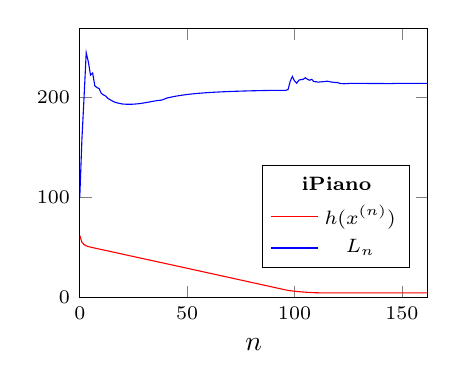
\begin{tikzpicture}
			\begin{axis}[%
					xlabel=$n$,
					xmin=0,
					xmax=162,
					ymin=0,
					height=5cm,
					width=6cm,
					legend style={at={(0.95,0.3)},anchor=east}
				]
				\addlegendimage{empty legend}
				\addlegendentry{\hspace{-.6cm}\textbf{iPiano}}
				%  %%%%%%%%%%%%%%%%%%%%%%%%%%%%%%%%%%%%%%%%%%%%%%%%%%%%%%%%%%%%
				\addplot[color=red] coordinates{
					(0,61.9284)
					(1,55.0942)
					(2,52.8104)
					(3,51.5286)
					(4,50.8406)
					(5,50.2876)
					(6,49.7831)
					(7,49.2999)
					(8,48.8285)
					(9,48.3644)
					(10,47.8984)
					(11,47.4317)
					(12,46.965)
					(13,46.4965)
					(14,46.0267)
					(15,45.5559)
					(16,45.0841)
					(17,44.6116)
					(18,44.139)
					(19,43.6663)
					(20,43.1937)
					(21,42.7214)
					(22,42.2497)
					(23,41.7785)
					(24,41.308)
					(25,40.8383)
					(26,40.3693)
					(27,39.901)
					(28,39.4335)
					(29,38.9666)
					(30,38.5003)
					(31,38.0343)
					(32,37.5685)
					(33,37.1025)
					(34,36.6362)
					(35,36.1691)
					(36,35.7009)
					(37,35.2314)
					(38,34.7606)
					(39,34.2897)
					(40,33.8195)
					(41,33.3495)
					(42,32.8795)
					(43,32.4094)
					(44,31.9393)
					(45,31.4692)
					(46,30.9989)
					(47,30.5285)
					(48,30.0581)
					(49,29.5875)
					(50,29.117)
					(51,28.6463)
					(52,28.1756)
					(53,27.7048)
					(54,27.234)
					(55,26.763)
					(56,26.292)
					(57,25.8209)
					(58,25.3498)
					(59,24.8786)
					(60,24.4072)
					(61,23.9358)
					(62,23.4644)
					(63,22.9928)
					(64,22.5212)
					(65,22.0496)
					(66,21.5778)
					(67,21.106)
					(68,20.6341)
					(69,20.1622)
					(70,19.6901)
					(71,19.2181)
					(72,18.7459)
					(73,18.2738)
					(74,17.8015)
					(75,17.3292)
					(76,16.8568)
					(77,16.3844)
					(78,15.9119)
					(79,15.4394)
					(80,14.9668)
					(81,14.4942)
					(82,14.0215)
					(83,13.5487)
					(84,13.0759)
					(85,12.6031)
					(86,12.1302)
					(87,11.6573)
					(88,11.1843)
					(89,10.7113)
					(90,10.2382)
					(91,9.76508)
					(92,9.29182)
					(93,8.81845)
					(94,8.34497)
					(95,7.87138)
					(96,7.40974)
					(97,7.01056)
					(98,6.69462)
					(99,6.42987)
					(100,6.18403)
					(101,5.95454)
					(102,5.74638)
					(103,5.55434)
					(104,5.37824)
					(105,5.21127)
					(106,5.05771)
					(107,4.92417)
					(108,4.80774)
					(109,4.71376)
					(110,4.6422)
					(111,4.59906)
					(112,4.57173)
					(113,4.55306)
					(114,4.53847)
					(115,4.52638)
					(116,4.51568)
					(117,4.50575)
					(118,4.4963)
					(119,4.48724)
					(120,4.4801)
					(121,4.47573)
					(122,4.47269)
					(123,4.47044)
					(124,4.46877)
					(125,4.4675)
					(126,4.4665)
					(127,4.46569)
					(128,4.46501)
					(129,4.46442)
					(130,4.4639)
					(131,4.46345)
					(132,4.46303)
					(133,4.46266)
					(134,4.46231)
					(135,4.462)
					(136,4.46172)
					(137,4.46145)
					(138,4.46121)
					(139,4.46099)
					(140,4.46078)
					(141,4.4606)
					(142,4.46042)
					(143,4.46026)
					(144,4.46012)
					(145,4.46003)
					(146,4.45996)
					(147,4.45992)
					(148,4.45989)
					(149,4.45986)
					(150,4.45985)
					(151,4.45984)
					(152,4.45983)
					(153,4.45982)
					(154,4.45982)
					(155,4.45982)
					(156,4.45981)
					(157,4.45981)
					(158,4.45981)
					(159,4.45981)
					(160,4.45981)
					(161,4.45981)
					(162,4.4598)
				};
				\addlegendentry{$h(x^{(n)})$}
				%-%
				%  %%%%%%%%%%%%%%%%%%%%%%%%%%%%%%%%%%%%%%%%%%%%%%%%%%%%%%%%%%%%
				\addplot[color=blue] coordinates{
					(0,100)
					(1,158.024)
					(2,200.18)
					(3,244.6)
					(4,235.454)
					(5,222.215)
					(6,224.275)
					(7,211.492)
					(8,209.73)
					(9,208.735)
					(10,204.029)
					(11,202.369)
					(12,201.391)
					(13,199.104)
					(14,197.717)
					(15,196.549)
					(16,195.419)
					(17,194.671)
					(18,194.155)
					(19,193.694)
					(20,193.286)
					(21,193.154)
					(22,193.063)
					(23,193.009)
					(24,193.052)
					(25,193.161)
					(26,193.314)
					(27,193.517)
					(28,193.772)
					(29,194.071)
					(30,194.411)
					(31,194.785)
					(32,195.184)
					(33,195.593)
					(34,195.995)
					(35,196.37)
					(36,196.699)
					(37,196.966)
					(38,197.158)
					(39,197.848)
					(40,198.849)
					(41,199.478)
					(42,199.942)
					(43,200.404)
					(44,200.848)
					(45,201.237)
					(46,201.589)
					(47,201.925)
					(48,202.247)
					(49,202.547)
					(50,202.822)
					(51,203.076)
					(52,203.313)
					(53,203.534)
					(54,203.741)
					(55,203.935)
					(56,204.117)
					(57,204.288)
					(58,204.449)
					(59,204.601)
					(60,204.743)
					(61,204.879)
					(62,205.006)
					(63,205.127)
					(64,205.242)
					(65,205.351)
					(66,205.455)
					(67,205.553)
					(68,205.647)
					(69,205.737)
					(70,205.823)
					(71,205.904)
					(72,205.983)
					(73,206.058)
					(74,206.129)
					(75,206.198)
					(76,206.264)
					(77,206.328)
					(78,206.389)
					(79,206.447)
					(80,206.504)
					(81,206.558)
					(82,206.611)
					(83,206.662)
					(84,206.71)
					(85,206.758)
					(86,206.803)
					(87,206.847)
					(88,206.89)
					(89,206.931)
					(90,206.971)
					(91,206.998)
					(92,206.985)
					(93,206.991)
					(94,207.002)
					(95,207.003)
					(96,207.003)
					(97,207.921)
					(98,216.117)
					(99,220.812)
					(100,216.462)
					(101,214.134)
					(102,217.09)
					(103,217.789)
					(104,217.875)
					(105,219.549)
					(106,218.02)
					(107,217.075)
					(108,217.983)
					(109,215.616)
					(110,215.608)
					(111,215.151)
					(112,215.38)
					(113,215.609)
					(114,215.719)
					(115,216.101)
					(116,215.817)
					(117,215.325)
					(118,215.049)
					(119,214.853)
					(120,214.863)
					(121,213.949)
					(122,213.683)
					(123,213.583)
					(124,213.647)
					(125,213.806)
					(126,213.923)
					(127,213.956)
					(128,213.947)
					(129,213.928)
					(130,213.912)
					(131,213.898)
					(132,213.886)
					(133,213.872)
					(134,213.859)
					(135,213.845)
					(136,213.831)
					(137,213.817)
					(138,213.803)
					(139,213.789)
					(140,213.775)
					(141,213.761)
					(142,213.747)
					(143,213.734)
					(144,213.721)
					(145,213.725)
					(146,213.811)
					(147,213.869)
					(148,213.924)
					(149,213.94)
					(150,213.941)
					(151,213.945)
					(152,213.949)
					(153,213.953)
					(154,213.957)
					(155,213.96)
					(156,213.962)
					(157,213.963)
					(158,213.965)
					(159,213.965)
					(160,213.965)
					(161,213.966)
					(162,213.965)
				};
				\addlegendentry{$L_n$}
			\end{axis}
		\end{tikzpicture}
		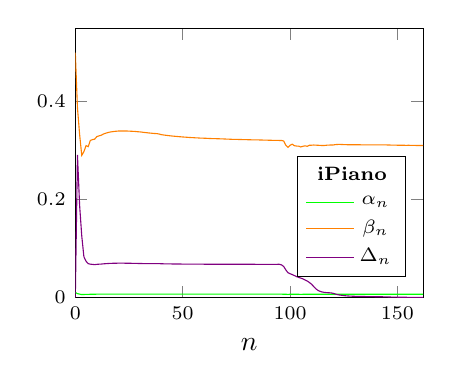
\begin{tikzpicture}
			\begin{axis}[%
					xlabel=$n$,
					xmin=0,
					xmax=162,
					ymin=0,
					height=5cm,
					width=6cm,
					legend style={at={(0.95,0.3)},anchor=east}
				]
				\addlegendimage{empty legend}
				\addlegendentry{\hspace{-.6cm}\textbf{iPiano}}
				%-%
				%  %%%%%%%%%%%%%%%%%%%%%%%%%%%%%%%%%%%%%%%%%%%%%%%%%%%%%%%%%%%%
				\addplot[color=green] coordinates{
					(0,0.009999)
					(1,0.00775131)
					(2,0.00666305)
					(3,0.00580436)
					(4,0.0059639)
					(5,0.00620958)
					(6,0.00617039)
					(7,0.00642403)
					(8,0.0064615)
					(9,0.00648293)
					(10,0.00658325)
					(11,0.00662004)
					(12,0.00664176)
					(13,0.00669282)
					(14,0.00672391)
					(15,0.00675074)
					(16,0.00677797)
					(17,0.00679593)
					(18,0.00680846)
					(19,0.00681984)
					(20,0.00683007)
					(21,0.00683349)
					(22,0.00683701)
					(23,0.00683863)
					(24,0.00683797)
					(25,0.00683578)
					(26,0.00683294)
					(27,0.0068281)
					(28,0.00682252)
					(29,0.00681627)
					(30,0.00680829)
					(31,0.00680032)
					(32,0.00679181)
					(33,0.00678263)
					(34,0.00677409)
					(35,0.00676608)
					(36,0.00675889)
					(37,0.00675382)
					(38,0.00674943)
					(39,0.00673411)
					(40,0.00671214)
					(41,0.00669822)
					(42,0.0066885)
					(43,0.0066785)
					(44,0.00666928)
					(45,0.00666095)
					(46,0.00665382)
					(47,0.00664672)
					(48,0.00663993)
					(49,0.00663364)
					(50,0.00662857)
					(51,0.00662332)
					(52,0.00661845)
					(53,0.00661423)
					(54,0.00660988)
					(55,0.00660648)
					(56,0.00660313)
					(57,0.00659992)
					(58,0.00659703)
					(59,0.00659361)
					(60,0.00659114)
					(61,0.00658852)
					(62,0.00658701)
					(63,0.00658471)
					(64,0.00658282)
					(65,0.00658033)
					(66,0.00657809)
					(67,0.00657659)
					(68,0.00657487)
					(69,0.00657356)
					(70,0.00657297)
					(71,0.00657215)
					(72,0.0065714)
					(73,0.00657038)
					(74,0.0065687)
					(75,0.00656816)
					(76,0.00656704)
					(77,0.0065663)
					(78,0.00656561)
					(79,0.00656465)
					(80,0.00656406)
					(81,0.00656351)
					(82,0.006563)
					(83,0.00656223)
					(84,0.00656148)
					(85,0.00656047)
					(86,0.00656011)
					(87,0.00656009)
					(88,0.00656011)
					(89,0.00655984)
					(90,0.0065596)
					(91,0.00656027)
					(92,0.00656117)
					(93,0.00656197)
					(94,0.00656266)
					(95,0.00656326)
					(96,0.00656419)
					(97,0.00654478)
					(98,0.0063741)
					(99,0.00628041)
					(100,0.00636825)
					(101,0.0064164)
					(102,0.00635669)
					(103,0.00634318)
					(104,0.00634258)
					(105,0.00630935)
					(106,0.00634079)
					(107,0.00636013)
					(108,0.0063421)
					(109,0.00639122)
					(110,0.00639138)
					(111,0.0064016)
					(112,0.00639719)
					(113,0.00639252)
					(114,0.00639078)
					(115,0.00638342)
					(116,0.00638972)
					(117,0.00639991)
					(118,0.00640585)
					(119,0.00640989)
					(120,0.00640997)
					(121,0.00642932)
					(122,0.00643467)
					(123,0.00643704)
					(124,0.006436)
					(125,0.00643359)
					(126,0.00643175)
					(127,0.00643135)
					(128,0.00643271)
					(129,0.00643311)
					(130,0.00643373)
					(131,0.00643431)
					(132,0.00643456)
					(133,0.00643571)
					(134,0.00643628)
					(135,0.0064371)
					(136,0.00643746)
					(137,0.0064379)
					(138,0.00643848)
					(139,0.00643906)
					(140,0.00643964)
					(141,0.00644021)
					(142,0.00644137)
					(143,0.00644194)
					(144,0.0064425)
					(145,0.00644271)
					(146,0.00644121)
					(147,0.00644088)
					(148,0.00644004)
					(149,0.00644028)
					(150,0.00644078)
					(151,0.00644112)
					(152,0.00644192)
					(153,0.00644212)
					(154,0.00644256)
					(155,0.00644234)
					(156,0.00644259)
					(157,0.00644372)
					(158,0.00644485)
					(159,0.00644543)
					(160,0.00644571)
					(161,0.00644628)
					(162,0.00644687)
				};
				\addlegendentry{$\alpha_n$}
				%-%
				%  %%%%%%%%%%%%%%%%%%%%%%%%%%%%%%%%%%%%%%%%%%%%%%%%%%%%%%%%%%%%
				\addplot[color=orange] coordinates{
					(0,0.5)
					(1,0.387555)
					(2,0.333094)
					(3,0.290126)
					(4,0.297888)
					(5,0.31007)
					(6,0.308069)
					(7,0.320685)
					(8,0.322413)
					(9,0.323323)
					(10,0.328415)
					(11,0.330086)
					(12,0.331138)
					(13,0.333651)
					(14,0.335285)
					(15,0.336572)
					(16,0.337726)
					(17,0.33845)
					(18,0.339053)
					(19,0.339517)
					(20,0.339923)
					(21,0.340042)
					(22,0.340011)
					(23,0.34004)
					(24,0.339956)
					(25,0.339796)
					(26,0.339483)
					(27,0.339323)
					(28,0.338994)
					(29,0.338513)
					(30,0.338197)
					(31,0.3377)
					(32,0.337107)
					(33,0.336683)
					(34,0.33609)
					(35,0.335673)
					(36,0.335266)
					(37,0.334864)
					(38,0.334646)
					(39,0.333836)
					(40,0.332581)
					(41,0.331926)
					(42,0.331345)
					(43,0.3308)
					(44,0.330245)
					(45,0.329783)
					(46,0.329332)
					(47,0.328932)
					(48,0.328547)
					(49,0.328187)
					(50,0.32779)
					(51,0.327481)
					(52,0.327192)
					(53,0.326822)
					(54,0.32658)
					(55,0.326353)
					(56,0.326027)
					(57,0.325858)
					(58,0.325554)
					(59,0.325472)
					(60,0.325254)
					(61,0.325077)
					(62,0.32481)
					(63,0.324648)
					(64,0.324396)
					(65,0.32436)
					(66,0.32425)
					(67,0.32408)
					(68,0.323947)
					(69,0.323787)
					(70,0.323567)
					(71,0.323383)
					(72,0.323203)
					(73,0.322994)
					(74,0.322999)
					(75,0.322829)
					(76,0.322727)
					(77,0.322595)
					(78,0.322466)
					(79,0.322372)
					(80,0.322248)
					(81,0.322126)
					(82,0.322006)
					(83,0.32192)
					(84,0.321836)
					(85,0.321787)
					(86,0.321674)
					(87,0.321531)
					(88,0.32139)
					(89,0.321282)
					(90,0.321176)
					(91,0.321019)
					(92,0.320969)
					(93,0.320866)
					(94,0.320758)
					(95,0.320693)
					(96,0.320597)
					(97,0.319603)
					(98,0.311223)
					(99,0.306604)
					(100,0.310757)
					(101,0.313016)
					(102,0.310013)
					(103,0.309264)
					(104,0.309056)
					(105,0.307393)
					(106,0.308791)
					(107,0.309688)
					(108,0.308765)
					(109,0.310976)
					(110,0.310984)
					(111,0.311345)
					(112,0.311086)
					(113,0.310859)
					(114,0.310625)
					(115,0.31027)
					(116,0.310427)
					(117,0.310969)
					(118,0.311213)
					(119,0.311409)
					(120,0.311368)
					(121,0.312158)
					(122,0.31251)
					(123,0.31258)
					(124,0.312484)
					(125,0.312231)
					(126,0.312051)
					(127,0.311986)
					(128,0.311871)
					(129,0.31189)
					(130,0.311875)
					(131,0.311858)
					(132,0.31187)
					(133,0.311789)
					(134,0.311772)
					(135,0.311662)
					(136,0.311667)
					(137,0.311735)
					(138,0.311718)
					(139,0.311701)
					(140,0.311684)
					(141,0.311667)
					(142,0.311587)
					(143,0.31157)
					(144,0.311551)
					(145,0.311516)
					(146,0.311399)
					(147,0.311247)
					(148,0.311162)
					(149,0.311083)
					(150,0.310958)
					(151,0.310976)
					(152,0.31088)
					(153,0.310844)
					(154,0.310716)
					(155,0.310799)
					(156,0.310765)
					(157,0.31064)
					(158,0.310514)
					(159,0.310452)
					(160,0.310421)
					(161,0.310358)
					(162,0.310297)
				};
				\addlegendentry{$\beta_n$}
				%-%
				%  %%%%%%%%%%%%%%%%%%%%%%%%%%%%%%%%%%%%%%%%%%%%%%%%%%%%%%%%%%%%
				\addplot[color=violet] coordinates{
					(0,-0.000364599)
					(1,0.29112)
					(2,0.188431)
					(3,0.125521)
					(4,0.0830333)
					(5,0.0738709)
					(6,0.0689289)
					(7,0.0679369)
					(8,0.0674423)
					(9,0.0669165)
					(10,0.0675091)
					(11,0.0678859)
					(12,0.0680741)
					(13,0.0685265)
					(14,0.068883)
					(15,0.0691719)
					(16,0.0694485)
					(17,0.0696419)
					(18,0.0697675)
					(19,0.0698584)
					(20,0.069932)
					(21,0.0699415)
					(22,0.0699245)
					(23,0.0698944)
					(24,0.0698413)
					(25,0.0697695)
					(26,0.0696822)
					(27,0.0695926)
					(28,0.0694934)
					(29,0.0693844)
					(30,0.0692828)
					(31,0.0691834)
					(32,0.0690892)
					(33,0.0690188)
					(34,0.0689643)
					(35,0.0689455)
					(36,0.068956)
					(37,0.0689982)
					(38,0.0690541)
					(39,0.0689863)
					(40,0.0687915)
					(41,0.0686534)
					(42,0.0685653)
					(43,0.0684898)
					(44,0.068418)
					(45,0.0683561)
					(46,0.0683031)
					(47,0.068253)
					(48,0.0682046)
					(49,0.0681588)
					(50,0.0681174)
					(51,0.0680799)
					(52,0.0680456)
					(53,0.0680094)
					(54,0.0679789)
					(55,0.0679562)
					(56,0.067928)
					(57,0.0679085)
					(58,0.0678839)
					(59,0.0678676)
					(60,0.0678502)
					(61,0.0678335)
					(62,0.0678178)
					(63,0.0678029)
					(64,0.0677843)
					(65,0.0677743)
					(66,0.0677632)
					(67,0.0677522)
					(68,0.0677416)
					(69,0.0677315)
					(70,0.0677219)
					(71,0.0677132)
					(72,0.0677048)
					(73,0.0676922)
					(74,0.0676878)
					(75,0.0676818)
					(76,0.0676753)
					(77,0.067669)
					(78,0.067663)
					(79,0.0676574)
					(80,0.0676521)
					(81,0.0676469)
					(82,0.067642)
					(83,0.0676373)
					(84,0.0676328)
					(85,0.0676285)
					(86,0.0676244)
					(87,0.0676206)
					(88,0.0676168)
					(89,0.0676135)
					(90,0.0676101)
					(91,0.0676095)
					(92,0.0676185)
					(93,0.0676263)
					(94,0.0676323)
					(95,0.0676399)
					(96,0.0664473)
					(97,0.0634335)
					(98,0.0563558)
					(99,0.0504509)
					(100,0.0484512)
					(101,0.0466692)
					(102,0.044658)
					(103,0.0425239)
					(104,0.0408775)
					(105,0.0394562)
					(106,0.0378493)
					(107,0.0356754)
					(108,0.033438)
					(109,0.0304092)
					(110,0.0269292)
					(111,0.0222727)
					(112,0.0176444)
					(113,0.01427)
					(114,0.0122985)
					(115,0.0110299)
					(116,0.0102373)
					(117,0.00975667)
					(118,0.00947644)
					(119,0.00927437)
					(120,0.00838955)
					(121,0.00705895)
					(122,0.00581927)
					(123,0.00495177)
					(124,0.0042562)
					(125,0.00368505)
					(126,0.00323513)
					(127,0.00289348)
					(128,0.00263187)
					(129,0.00242761)
					(130,0.00226444)
					(131,0.00213028)
					(132,0.00201653)
					(133,0.00191723)
					(134,0.0018283)
					(135,0.00174697)
					(136,0.00167164)
					(137,0.00160121)
					(138,0.00153457)
					(139,0.00147132)
					(140,0.00141093)
					(141,0.0013532)
					(142,0.00129802)
					(143,0.00124511)
					(144,0.00116703)
					(145,0.00102722)
					(146,0.000853786)
					(147,0.00070983)
					(148,0.000591104)
					(149,0.000493866)
					(150,0.000414036)
					(151,0.000348762)
					(152,0.000295921)
					(153,0.000253343)
					(154,0.000219127)
					(155,0.000191635)
					(156,0.000169635)
					(157,0.000151994)
					(158,0.000137841)
					(159,0.000126463)
					(160,0.000117236)
					(161,0.000109609)
					(162,0.00010332)
				};
				\addlegendentry{$\Delta_n$}
				%/%
			\end{axis}
		\end{tikzpicture}
	\end{subfigure}
	\caption{Convergence of iPiano. Shown is the value of the objective function $h(x{(n)})$ for each iterate $x{(n)}$, $n \geq 0$, as well as the corresponding parameters $\alpha_n$, $\beta_n$ and $L_n$. Furthermore, $\Delta_n := \|x^{(n)} - x^{(n - 1)}\|_2$ is shown.}
	\end{figure}
	\end{frame}
	
	\begin{frame}{Denoising -- Results (cont'd)}
		\begin{figure}[h]
			\centering
			\begin{subfigure}[t]{0.25\textwidth}
				\includegraphics[scale=0.175]{../paper/pictures/denoising/image/3096_tilde.png}
			\end{subfigure}
			\begin{subfigure}[t]{0.25\textwidth}
				\includegraphics[scale=0.175]{../paper/pictures/denoising/image/42049_tilde.png}
			\end{subfigure}
			\begin{subfigure}[t]{0.25\textwidth}
				\includegraphics[scale=0.175]{../paper/pictures/denoising/image/147091_tilde.png}
			\end{subfigure}
			\begin{subfigure}[t]{0.25\textwidth}
				\includegraphics[scale=0.175]{../paper/pictures/denoising/image/3096_ipiano_absolute.png}
			\end{subfigure}
			\begin{subfigure}[t]{0.25\textwidth}
				\includegraphics[scale=0.175]{../paper/pictures/denoising/image/42049_ipiano_absolute.png}
			\end{subfigure}
			\begin{subfigure}[t]{0.25\textwidth}
				\includegraphics[scale=0.175]{../paper/pictures/denoising/image/147091_ipiano_absolute.png}
			\end{subfigure}
			\begin{subfigure}[t]{0.25\textwidth}
				\includegraphics[scale=0.175]{../paper/pictures/denoising/image/3096_ipiano_squared.png}
			\end{subfigure}
			\begin{subfigure}[t]{0.25\textwidth}
				\includegraphics[scale=0.175]{../paper/pictures/denoising/image/42049_ipiano_squared.png}
			\end{subfigure}
			\begin{subfigure}[t]{0.25\textwidth}
				\includegraphics[scale=0.175]{../paper/pictures/denoising/image/147091_ipiano_squared.png}
			\end{subfigure}
			\caption{Image denoising experiment; noisy image in the top row, $\rho_{1,\text{abs}}$ in the middle row and $\rho_{1,\text{sqr}}$ in the bottom row.}
	\label{fig:image-denoising}
		\end{figure}
	\end{frame}
	
	\begin{frame}{Binary Segmentation -- Model}
		Binary segmentation based on an approximation of the Mumford-Shah model \cite{MumfordShah:1989,Shen:2005}; $u: [0,1]^2 \rightarrow  [-1,1]$:
		\begin{align}
			\begin{aligned}
				h_\epsilon(u; c_+, c_-, u^{(0)}, \lambda) =& \int_{\Omega} \left(9 \epsilon \|\nabla u(x)\|_2^2 + \frac{(1 - u(x)^2)^2}{64 \epsilon}\right) dx\only<2>{\begin{tikzpicture}[overlay]\draw[-,thick,RWTHblue] (0.1,-0.45) -- (-6.15,-0.45) -- (-6.15,0.75) -- (0.1,0.75) -- (0.1,-0.45);\end{tikzpicture}}\\
				& + \lambda \int_{\Omega}\left(\frac{1 + u(x)}{2}\right)^2(u^{(0)}(x) - c_+)^2 dx\only<3>{\begin{tikzpicture}[overlay]\draw[-,thick,RWTHblue] (0.1,-1.55) -- (-6.4,-1.55) -- (-6.4,0.65) -- (0.1,0.65) -- (0.1,-1.55);\end{tikzpicture}}\\
				& + \lambda \int_{\Omega} \left(\frac{1 - u(x)}{2}\right)^2 (u^{(0)}(x) - c_-)^2 dx.
			\end{aligned}
		\end{align}
		
		\pause
		(It can be shown, that for $\epsilon \rightarrow 0$,
		\begin{align}
			\int_{\Omega} \left(9 \epsilon \|\nabla u(x)\|_2^2 + \frac{(1 - u(x)^2)^2}{64 \epsilon}\right) dx
		\end{align}
		approximates $|u|_{BV}$.)
	\end{frame}
	
	\begin{frame}{Binary Segmentation -- Results (cont'd)}
		\begin{figure}
			\centering
			\begin{subfigure}[t]{0.215\textwidth}
				\includegraphics[scale=0.15]{../paper/pictures/3096.jpg}
			\end{subfigure}
			\begin{subfigure}[t]{0.215\textwidth}
				\includegraphics[scale=0.15]{../paper/pictures/segmentation/squared/{3096_-0.200000_seg}.png}
			\end{subfigure}
			\begin{subfigure}[t]{0.215\textwidth}
				\includegraphics[scale=0.15]{../paper/pictures/segmentation/squared/{3096_0.000000_seg}.png}
			\end{subfigure}
			\begin{subfigure}[t]{0.215\textwidth}
				\includegraphics[scale=0.15]{../paper/pictures/segmentation/squared/{3096_0.200000_seg}.png}
			\end{subfigure}
			\vskip 2px
			%%%%%%%%%%%%%%%%%%%%%%%%%%%%%%%%
			\begin{subfigure}[t]{0.215\textwidth}
				\includegraphics[scale=0.15]{../paper/pictures/42049.jpg}
			\end{subfigure}
			\begin{subfigure}[t]{0.215\textwidth}
				\includegraphics[scale=0.15]{../paper/pictures/segmentation/squared/{42049_-0.200000_seg}.png}
			\end{subfigure}
			\begin{subfigure}[t]{0.215\textwidth}
				\includegraphics[scale=0.15]{../paper/pictures/segmentation/squared/{42049_0.000000_seg}.png}
			\end{subfigure}
			\begin{subfigure}[t]{0.215\textwidth}
				\includegraphics[scale=0.15]{../paper/pictures/segmentation/squared/{42049_0.200000_seg}.png}
			\end{subfigure}
			\vskip 2px
			%%%%%%%%%%%%%%%%%%%%%%%%%%%%%%%%
			\begin{subfigure}[t]{0.215\textwidth}
				\includegraphics[scale=0.15]{../paper/pictures/147091.jpg}
			\end{subfigure}
			\begin{subfigure}[t]{0.215\textwidth}
				\includegraphics[scale=0.15]{../paper/pictures/segmentation/squared/{147091_-0.200000_seg}.png}
			\end{subfigure}
			\begin{subfigure}[t]{0.215\textwidth}
				\includegraphics[scale=0.15]{../paper/pictures/segmentation/squared/{147091_0.000000_seg}.png}
			\end{subfigure}
			\begin{subfigure}[t]{0.215\textwidth}
				\includegraphics[scale=0.15]{../paper/pictures/segmentation/squared/{147091_0.200000_seg}.png}
			\end{subfigure}
			\vskip 2px
			\caption{Segmentation results for thresholds $\tau = -0.2, 0.0, 0.2$ and using $g_{\text{sqr}}$; the foreground segment $S_f$ is depicted in white.}
			\label{fig:segmentation}
		\end{figure}
	\end{frame}
	
	\section{Conclusion}
	\begin{frame}{Conclusion}
		We discussed the minimization of composite functions of the form
		\begin{align}
			\min_{x \in \mathbb{R}^d} h(x) = \min_{n \in \mathbb{R}^d} (f(x) + g(x)).
		\end{align}
		\vskip 1em
		
		\pause
		Ochs \etal \cite{OchsChenBroxPock:2013} proposed the iPiano algorithm to solve this problem under to following requirements:
		\begin{enumerate}[label=--]
			\item $g$ proper closed convex and lower semi continuous;
			\item $f \in C^1$ with $L$-Lipschitz continuous $\nabla f$;
			\item $h$ coercive and bounded below;
			\item and $H_{\delta_n}(x^{(n)}, x^{(n - 1)}) = h(x^{(n)}) + \delta_n \Delta_n$ satisfying the Kurdyka-Lojasiewicz property \cite{Lojasiewicz:1993,Kurdyka:1998} at a critical point.
		\end{enumerate}
		\vskip 1em
		
		\pause
		The algorithm can be implemented efficiently in C++ and used to solve image processing tasks.
	\end{frame}
	
	\begin{frame}{Appendix -- Kurdyka-Lojasiewicz Property}
		\begin{definition}
			$H$ has the Kurdyka-Lojasiewicz property at point $\tilde{z} \in \dom(\partial H)$ there exist $\eta \in (0,\infty]$, a neighborhood $U$ of $\tilde{z}$, and a continuous concave function $\phi : [0, \eta) \rightarrow \mathbb{R}_{+}$ such that
			\begin{itemize}
				\item[--] $\phi \in C^1((0, \eta))$, $\phi(0) = 0$, and for all $s \in (0, \eta)$, $\phi'(s) > 0$;
				\item[--] and for all $z \in U \cap \{z \in \mathbb{R}^{2d} | H(\tilde{z}) < H(z) < H(\tilde{z}) + \eta\}$ the Kurdyka-Lojasiewicz inequality holds:
			\end{itemize}
			\begin{align}
				\phi'(H(z) - H(\tilde{z})) \inf_{\hat{z} \in \partial H(z)}\|\hat{z}\|_2 \geq 1.\only<2>{\begin{tikzpicture}[overlay]\draw[-,thick,RWTHblue] (0.25,-0.45) -- (-6,-0.45) -- (-6,0.65) -- (0.25,0.65) -- (0.25,-0.45);\end{tikzpicture}}\label{eq:kl-inequality}
			\end{align}
		\end{definition}
		\vskip 1em
		
		\pause
		Intuitively, for $H \in C^1$, this means that $\phi$ has to be steep around critical points $\tilde{z}$ of $H$ where $\nabla H$ is flat.
	\end{frame}
	
	\bibliographystyle{alpha}
	\bibliography{slides}
\end{document}